\section{Can deformation be allowed to fix everything?}
\label{sec:deformation-freedom}

\begin{figure}[!htb]
\centering
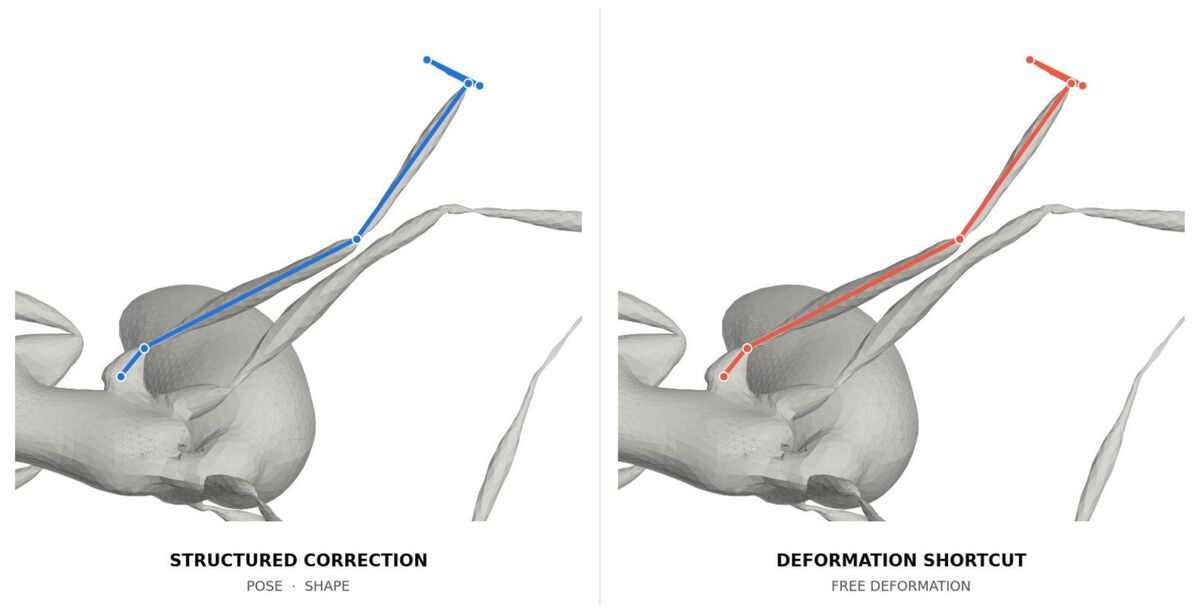
\includegraphics[width=0.58\linewidth]{figures/fig_deformation_shortcut.jpg}
\caption{What happens when the model has enough freedom to make the surface
look right regardless of pose. Left: a structured correction, achieved
through the model's own pose and shape parameters. Right: the same visual
improvement achieved by free per-vertex deformation, which bends the leg
rather than re-posing the joint.}
\label{fig:deformation-shortcut}
\end{figure}

The registration objective includes free per-vertex deformation terms,
bounded only by edge-length and Laplacian regularisation
(\S\ref{sec:registration}), because the model's fixed shape space cannot by
itself represent every idiosyncrasy of a real specimen. This freedom is
also, mechanically, an escape hatch: a joint that is posed incorrectly can
be visually corrected either by rotating it to the right angle, or by
bending the mesh around a wrong angle until the surface distance term is
satisfied anyway (Figure~\ref{fig:deformation-shortcut}). The two solutions
can be nearly indistinguishable by $\mathcal{L}_{\mathrm{chamfer}}$ while
being anatomically unrelated: only the first preserves the correspondence
that makes the fit usable for measurement (Chapter~\ref{ch:validation}).

This is the same mechanism as \F{F1} (\S\ref{sec:geometric-agreement}),
observed at the level of a single joint rather than a whole specimen, and it
is why deformation cost is treated in the delivered recipe as a
\emph{regularising} penalty rather than a free parameter: neither an
unbounded deformation budget nor a frozen one is correct, because the
optimum that best serves anatomical correctness sits in between the two
(\S\ref{sec:three-failure-modes}).
